\documentclass{article}

\usepackage{amsmath,amssymb}
\usepackage{fullpage}
\usepackage{mathtools}
\usepackage{enumerate}
\usepackage{hyperref}
\usepackage{graphicx}
\graphicspath{{../logos/}}


\begin{document}

\setlength{\tabcolsep}{6pt}
\begin{center} \begin{tabular}{cccc}
	
\includegraphics[height=56pt]{SAMF_logo.jpg} &
	
\includegraphics[height=56pt]{SAICA_logo.jpg} &
	
\includegraphics[height=56pt]{OM_Logo_Stacked_Vignette_on_White_RGB.jpg} &
	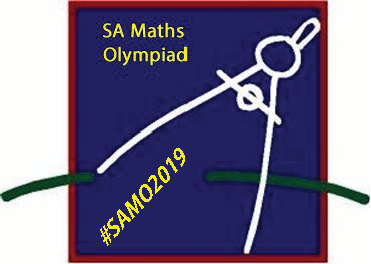
\includegraphics[height=56pt]{SAMO2019.png}
\end{tabular} \end{center}


\bigskip


\begin{center}
	\textbf{\Large Senior Another Monthly Problem Set Solutions}
\end{center}

\begin{enumerate}

\medskip
\item[1.] % 2015 Azerbaijan IMO TST Q1, A(N)
{\itshape A set $A = \{a_1, a_2, \dotsc, a_n\}$ of distinct positive integers is called \emph{powerful} if
\[ \prod_{i \neq j} a_j \mid a_i^{2020} \]
for all $i \in \{1, 2, \dotsc, n\}$.
Find all $n \ge 3$ such that there exists a powerful set containing exactly $n$ elements.}

%\item[1. ANS]
For $n\leq2020$, consider the set of unique primes $(p_1,p_2,...,p_n)$ and let $P = \prod_{i=1}^{n} p_i$. Let $a_i = Pp_i$. We now show that this set is $powerful$.

$\prod_{j=1}^{n} a_j \mid {a_i}^{2021} \iff P^{n+1} \mid P^{2021}p_i^{2021}$, which is true.
For $n>2020$ let $a_i$ be the minimal value in the $powerful$ set $A$.
But ${a_i}^{2021} \leq \prod_{j=1}^{n} a_i < \prod_{j=1}^{n} a_j \leq {a_i}^{2020}$, which is a contradiction.


\medskip
\item[2.] % All Russian Olympiad 2017 Grade 10 Q2, G
{\itshape Let $ABC$ be an acute angled isosceles triangle with $AB = AC$ and circumcentre $O$.
Lines $BO$ and $CO$ intersect $AC$ and $AB$ at $D$ and $E$ respectively.
A straight line $l$ is drawn through $E$ parallel to $AC$.
Prove that the line $l$ is tangent to the circumcircle of $\triangle DOC$.}

%\item[2. ANS]
Note that $AO$ is a line of symmetry that maps $B\rightarrow C$ and $D\rightarrow E$. Let $l$ and it's reflection $k$ intersect on $AO$ at $F$.
Note $AC \parallel EF, AB \parallel DF$ and $AE=AD$ meaning $ADFE$ is a rhombus $\implies \angle AFD = \angle FAD = \angle OAC$.
Additionally as $O$ is the circumcentre, $OA = OC \implies \angle OCA = \angle OAC = \angle AFD \implies ODCF$ cyclic.
And since $EF \parallel AC\implies\angle EFD = \angle FDC\implies l$ tangent to the circumcircle of $\triangle DOC$


\medskip
\item[3.] % 2017 Princeton University Maths Competition A4, A
{\itshape Let the sequence $a_1$, $a_2$, $\dotsc$ be defined by $a_n = 11 a_{n - 1} - n$.
Find the smallest possible value of $a_1$ such that $a_i > 0$ for all $i \in \mathbb{N}$.}

Let $b_n = a_{n + 1} - a_n$. Then, we have
\begin{align*}
	b_n &= 10a_n - (n + 1) \\
	 &= 10(11a_{n - 1} - n) - (n + 1) \\
	 &= 11(10a_{n - 1} - n) - 1 \\
	 &= 11b_{n - 1} - 1
\end{align*}

Therefore, if $b_1 < \frac{1}{10}$, then the sequence $b_1$, $b_2$, $\dots$ is decreasing, and in fact becomes arbitrarily small, which means that the sequence $a_1$, $a_2$, $\dots$ becomes arbitrarily small as well. Therefore, $b_1 \ge \frac{1}{10}$, so we have $a_2 - a_1 \ge \frac{1}{10}$, or equivalently $a_1 \ge \frac{21}{100}$. Since the sequence $a_1$, $a_2$, $\dots$ is increasing if $a_1 = \frac{21}{100}$, this is our answer.

\medskip
\item[4.] % China Southeast Math Olympiad 2014, Q2, C
{\itshape There are $n \ge 4$ people at a fencing competition.
Each player plays against every other player exactly once, and there are no draws.
The organisers decide that the competition is representative if they can find $4$ people, $a_1$, $a_2$, $a_3$, and $a_4$, such that $a_i$ beats $a_j$ whenever $i < j$.
Find the smallest value $n$ such that the competition will always be representative.}

%\item[4. ANS]
Let $S = (a_1,a_2,...,a_n)$ be a directed graph where there is a edge from $a_i$ to $a_j$ if and only if $a_i$ beats $a_j$. Note that if $S$ is $non-representative$ then $a_1,...,a_{n-1}$ is also $non-representative$. A construction for a $non-representative$ graph $S$ for $n=7$ is as follow: $a_i$ beats $a_{i+1}$, $a_{i+2}$ and $a_{i+4}$, where $a_j = a_{j-7}$ if $j>7$. For $n=8$ let $A$ be the set of people $a_1$ beats or loses to in $S$, whichever is greater. By Pigeon Hole Principal there are at least $\lceil{\frac{7}{2}}\rceil$ people in $A$, without loss of generality let $A$ be the set of people $a_1$ beats and have it include $a_2$. Similarly, let $B$ be the set of people $a_2$ beats or loses to in $A$, whichever is greater. There are at least $\lceil{\frac{3}{2}}\rceil$ people in $B$, without loss of generality let $B$ be the set of people $a_2$ beats and have it include $a_3$ and $a_4$. Note that $a_1$ beats $a_2$, $a_3$ and $a_4$; $a_2$ beats $a_3$ and $a_4$; without loss of generality $a_3$ beats $a_4$, meaning $S$ is always $representative$ for $n=8$


\medskip
\item[5.] % 2011 Japan Mathematical Olympiad Finals Problem 5, G
{\itshape Given some $4$ points in the plane, one can construct $4$ different triangles with vertices amongst the $4$ points.
If the inscribed circles of these $4$ triangles all have the same radius, show that the $4$ triangles are congruent. }

%\item[5. ANS]
Let $A,B,C,D$ be the $4$ points in a clockwise order and let $I_A$ be the in-centre of $\triangle ABD$, similarly define $I_B$,$I_C$ and $I_D$. Let $A_1$,$A_2$ and $A_3$ be the tangency points of the in-circle with centre $I_A$ to sides $AB$,$BD$ and $DA$ respectively. Similarly define the other tangency points. 

Note that $A_1B = A_2B$, $A_3D = A_2D$, $B_1B = B_3B$ and $D_1D = D_3D$
\begin{align*}
	\implies B_3B+A_1B_3+A_3D_1+D_1D &= A_1B+A_3D = A_2B+A_2D = BD \\
	= C_2B+C_2D = C_3B+C_1D &= B_1B+C_3B_1+C_1D_3+D_3D \\
	\implies A_1B_3 + A_3D_1 &= C_3B_1+C_1D_3
\end{align*}
Similarly but using diagonal $AC$ instead of $BD$ we get that
\[ B_1C_3 + B_3A_1 = D_3C_1 + D_1A_3 \implies A_1B_3 = C_1D_3\ \text{and}\ D_1A_3 = B_1C_3. \]
Now note that $D_1A_3 = I_DI_A$ as $I_AA_3 = r = I_DD_1$ and $I_AA_3 \parallel I_DD_1$, similarly for $I_AI_B$,$I_BI_C$ and $I_CI_D$.
Hence we have $I_DI_A=D_1A_3=B_1C_3=I_BI_C$, and similarly $I_AI_B=I_CI_D \implies I_AI_BI_CI_D$ is a parallelogram $\implies ABCD$ is a parallelogram. 
Finally note that
\begin{align*}
	rBD &= \frac{r(AB+BD+BA)}{2} + \frac{r(CD+DB+BC)}{2} = |ABD|+|CDB| = |ABCD| \\
	&= |BCA|+|DAC| = \frac{r(BC+CA+AB)}{2} + \frac{r(DA+AC+CD)}{2} = rAC \\
	\implies BD &= AC;
\end{align*}
so $ABCD$ is a rectangle, which satisfies the condition.


\medskip
\item[6.] % Emile Tredoux 2020, N(G)
{\itshape Your second favourite thing in this world is Table Mountain, how perfectly horizontal the top of it is.
Your favourite thing in this world is, of course, Mathematics.
Hence, for your birthday you received $n-2$ regular polygons, with number of sides $3, 4, \dotsc, n$ respectively.
You want to combine your two favourite things by stacking all of your polygons on top of each other such that any two consecutively placed polygon share an edge.
For which values of $n$ can you stack your polygon such that the top of your stack is perfectly flat like the top of Table Mountain?
i.e. the top-most edge and bottom-most edge of your stack are parallel.}

%\item[6. ANS] % Emile Tredoux 2020
Let $E_0,E_1,...,E_{n-2}$ be the set of shared edges in your stack, with $E_i$ being the edge that's shared between the $i^{th}$ and $i+1^{th}$ placed polygons, and with $E_0$ and $E_{n-2}$ being the bottom- and top-most edge respectively.

Note that the edges of a regular $p-gon$ are just rotated by an integer multiple of $\frac{360}{p}$ degrees, therefore edge $E_i$ is just $E_{i-1}$ rotated by some positive integer multiple $a_q < q$ of $\frac{360}{q}$, where $q$ is the number of sides of the polygon shared by $E_i$ and $E_{i-1}$.
Let this multiple be called $q_i$ for $0<i<n-2$

Therefore the angle of inclination of $E_{n-2}$ is just some sum of these $q_i$ mod $180$.
For $E_{n-2}$ to be perfectly flat, this value must equal $0$.

\[ \sum_{i=1}^{n-2} q_i \equiv_{180} 0 \implies {\sum_{i=3}^{n} \frac{a_i}{i} \equiv_{1} 0} \]

Let $p$ be the largest prime less than or equal to $n$.
Note that $\frac{a_p}{p} + \frac{a_i}{i}$ will always have a fractional part with denominator some multiple of $p$ unless $gcd(p,i) \neq 1$, meaning $i \geq 2p$, which by Bertrand's postulate implies that there exists some prime $q$ such that $p < q < 2p$, which is a contradiction.

Therefore no $n$ exist to satisfy the condition in the question statement.

\medskip
\item[7.]% SAMO Longlist JM-2014-1, N
{\itshape Let $\mathbb{N}$ denote the set of positive integers.

Consider the function $f : \mathbb{N} \times \mathbb{N} \to \{-1,1\}$, defined as follows:
\[ f(i,j) = \begin{dcases*} -1 & if $i = 1$ or $j = 1$ \\ f(i-1,j) \cdot f(i,j-1) & if $i > 1$ and $j > 1$ \end{dcases*}. \]
Determine the largest $i \leq 2015$ such that $f(i,2015) = -1$.}

We shall use double induction to get the function into a closed form that allows us to calculate arbitrary terms easily.

\textbf{Induction Hypothesis 1:} The function is given by
$$f(i, j) = (-1)^{\binom{i + j - 2}{i - 1}}. $$
for all $i$, $j$ $\in \mathbb{N}$.

\textbf{Base Case 1: $i = 1$:} By definition, we have $f(i, j) = -1$. Notice that $\binom{i + j - 2}{i - 1} = \binom{i + j - 2}{0} = 1$. Thus, we have that
$$LHS = f(i, j) = -1 = (-1)^1 = (-1)^{\binom{i + j - 2}{i - 1}} = RHS.$$
So the base case is true.

\textbf{Inductive Step 1:} Assume that Induction Hypothesis 1 is true for $i = k \in \mathbb{N}$. We shall prove that it is also true for $i = k + 1$. To do this, we shall perform induction on $j$.

\begin{quote}
\textbf{Induction Hypothesis 2:} The function is given by
$$f(k + 1, j) = (-1)^{\binom{(k + 1) + j - 2}{(k + 1) - 1}}. $$
for all $j$ $\in \mathbb{N}$ with $k$ being a fixed value such that Induction Hypothesis 1 holds for $i = k$.

\textbf{Base Case 2: $j = 1$:} By definition, we have $f(k + 1, j) = -1$. Notice that $\binom{(k + 1) + j - 2}{(k + 1) - 1} = \binom{k}{k} = 1$. Thus, we have that
$$LHS = f(k + 1, j) = -1 = (-1)^1 = (-1)^{\binom{(k + 1) + j - 2}{(k + 1) - 1}} = RHS.$$
So the base case is true.

\textbf{Inductive Step 2:} Assume that Induction Hypothesis 2 is true for $j = m \in \mathbb{N}$. We shall prove that it is true for $j = m + 1$ as well.

We have that $f(k + 1, m + 1) = f(k, m + 1) \cdot f(k + 1, m)$. From Induction Hypothesis 1 we have that 
$$f(k, m + 1) = (-1)^{\binom{k + (m + 1) - 2}{k - 1}} = (-1)^{\binom{k + m - 1}{k - 1}}.$$
From Induction Hypothesis 2 we have that
$$f(k + 1, m) = (-1)^{\binom{(k + 1) + m - 2}{(k + 1) - 1}} = (-1)^{\binom{k + m - 1}{k}}.$$

Putting these together we get that

$$f(k + 1, m + 1) = (-1)^{\binom{k + m - 1}{k - 1}} \cdot (-1)^{\binom{k + m - 1}{k}} = (-1)^{\binom{k + m}{k}} = (-1)^{\binom{(k + 1) + (m + 1) - 2}{(k + 1) - 1}}$$

so indeed, we have that if the formula holds for $j = m$, it must also be true for $j = m + 1$. So by the Principle of Mathematical Induction, Induction Hypothesis 2 is true for all $j \in \mathbb{N}$ and $k$ is some fixed value.
\end{quote}

Coming back to the first induction, we now have that if Induction Hypothesis 1 is true for $i = k$, then indeed, we have that
\[ f(k + 1, j) = (-1)^{\binom{(k + 1) + j - 2}{(k + 1) - 1}} \quad \forall j \in \mathbb{N}, \]
which is what was required to prove from Induction Step 1.
Thus, by the Principle of Mathematical Induction, we also have that Induction Hypothesis 1 is true for all $i \in \mathbb{N}$.

We have thus reduced the problem from determining when $f(i, 2015) = -1$ to when $\displaystyle \binom{i + 2015 - 2}{i - 1} = \binom{i + 2013}{i - 1}$ is odd.

$$\binom{i + 2013}{i - 1} = \frac{(i + 2013)!}{(i - 1)!(2014)!}.$$

For this expression to be odd, we need the highest power of two dividing the numerator to be the same as the highest power of two dividing the denominator. This statement is equivalent to
$$\sum_{r = 1}^{\infty} \left\lfloor{\frac{i + 2013}{2^r}}\right\rfloor = \sum_{r = 1}^{\infty} \left\lfloor \frac{i - 1}{2^r} \right\rfloor + \left\lfloor \frac{2014}{2^r} \right\rfloor.$$

Since $\left\lfloor a + b \right\rfloor \ge \left\lfloor a \right\rfloor + \left\lfloor b \right\rfloor$ for all $a, b \in \mathbb{R}$, the above equality holds if and only if equality holds in each term. Notice that for $i \le 2015$,
\[ \left\lfloor \frac{i + 2013}{2^{11}} \right\rfloor = \left\lfloor \frac{i - 1}{2^{11}} \right\rfloor + \left\lfloor \frac{2014}{2^{11}} \right\rfloor \iff i + 2013 < 2^{11} \iff i < 35 \iff i \le 34. \]
From here it is an exercise in arithmetic to confirm that $i = 34$ does indeed satisfy the equality of the infinite sums.

Thus $i = 34$ is the largest value of $i$ such that $f(i, 2015) = -1$.

\medskip
\item[8.] % Moscow Olympiad 1996 59.9.5, C
{\itshape Ali-Baba and a robber divide a treasure consisting of 100 golden coins, which is initially split into 10 piles of 10 coins each.

Ali-Baba chooses 4 piles, places a mug beside each pile, and puts several coins (at least $1$, but not the whole pile) from the respective pile into each mug.
The robber must permute the mugs, after which the coins are taken out from each mug and added to its newly associated pile.
Then Ali-Baba again selects 4 piles of 10, places mugs beside the piles, etc.

At any moment Ali-Baba can quit and go away with any 3 mugs he chooses, the remaining coins being the robber's share.
What is the greatest number of coins Ali-Baba can guarantee to collect?}

\textit{(Solution by Kgaogelo Bopape)}
First we show that Ali-Baba can take at least $72$ coins by applying the following
procedure:
	
If the four biggest piles have at least $5$ coins, then choose those piles. If not then we are done and Ali-Baba can take the three piles with the most stones.
Let the four piles with the most coins be $A$, $B$, $C$ and $D$ respectively (arranged from most to least).
Take $1$ coin from pile $A$, $2$ coins from pile $B$, $3$ coins from pile $C$ and $4$ coins from pile $D$.
Let there be $A_i$, $B_i$, $C_i$, $D_i$ coins in the piles before the iteration of the procedure and $A_f$, $B_f$, $C_f$, $D_f$ coins after the iteration of the procedure.
Clearly, $A_f \ge A_i$.
If $A_f = A_i$, then $B_f \ge B_i \implies A_f + B_f \ge A_i + B_i$.
If $A_f > A_i$, then $A_f \ge A_i + 1$ and $1 \ge B_i - B_f \implies A_f + B_f \ge A_i + B_i$.
$A_i + B_i + C_i + D_i = A_f + B_f + C_f + D_f$ and $D_i \ge D_f \implies A_f + B_f + C_f \ge A_i + B_i + C_i$
Hence:
$$A_f \ge A_i$$
$$A_f + B_f \ge A_i + B_i$$
$$A_f + B_f + C_f \ge A_i + B_i + C_i$$
If all the above inequalities become equalities then, $A_f = A_i$, $B_f = B_i$, $C_f = C_i$, $D_f = D_i$ which is not possible.
Let the three piles with the most coins have $W$, $X$ and $Y$ coins respectively.
$$W \ge A_f$$
$$W + X \ge A_f + B_f$$
$$W + X + Y \ge A_f + B_f + C_f$$
$$3W + 2X + Y \ge 3A_f + 2B_f + 2C_f > 3A_i + 2B_i + C_i$$
$\implies$ the quantity $Z = 3W + 2X + Y$ strictly increases after each iteration of the procedure. Also notice that $3(W + X + Y) > 3W + 2X + Y$, so the procedure ends either when $3(W + X + Y ) = 216$ or smallest $7$ piles all have at most $4$ coins. Either way, Ali-Baba can always take $72$ coins.

Now we will show that the robber can always take at least $28$ coins if the robber applies the following procedure:

Assume that Alibaba chooses piles with $A_1$, $A_2$, $A_3$ and $A_4$ coins and removes $b_1$, $b_2$, $b_3$ and $b_4$ coins from the piles. Suppose $b_i = b_j$ for some $i$, $j$ ($i \ne j$), where $b_i$ coins were removed from the pile with $A_m$ coins and $b_j$ coins were removed from the pile with $A_n$ coins ($m \ne n$). The robber can just place the mug with $b_i$ coins beside the pile which had $A_n$ coins and the mug with $b_j$ coins beside the pile which had $A_m$ coins and place the other mugs next to the piles from which they came. Then the state of the piles remains the same.

Now assume that immediately after the coins were removed, $c_1$, $c_2$, $c_3$ and $c_4$ remained in the piles. Suppose $c_i = c_j$ for some $i$, $j$ ($i \ne j$), and $c_i$ coins remained from the pile which had $A_m$ coins and $c_j$ coins remained from the pile which had $A_n$ coins ($m \ne n$), and that $b_p$ coins were removed from the pile which had $A_m$ coins and $b_q$ coins were removed from the pile which had $A_n$ coins. Then the robber can just place the mug with $b_p$ coins beside the pile with $c_j$ remaining coins and the mug with $b_q$ coins beside the pile with $c_i$ remaining coins and place the other mugs next to the piles from which they came. Then the state of the piles remains the same.

Without loss of generality assume $b_4 > b_3 > b_2 > b_1 \ge 1$ and $c_4 > c_3 > c_2 > c_1 \ge 1$. Notice that $b_i \ge i$ and $c_i \ge i$ for all $i$ ($1 \le i \le 4$) so you can either choose $(b_i + c_{5-i} )$ for all $i$ or
$$(b_1 + c_4 )$$
$$(b_2 + c_3 )$$
$$(b_3 + c_2 )$$
$$(b_4 + c_1 )$$
depending on which is the identity permutation. This means that after every iteration of the procedure, the number of piles with less than $4$ coins does not increase. Since there are initially no coins with $4$ coins. The total number of coins of the $7$ smallest piles is at least $28$.

Hence the maximum amount of coins Ali-Baba is guaranteed to collect is $72$.
\end{enumerate}

\end{document}
